% Options for packages loaded elsewhere
\PassOptionsToPackage{unicode}{hyperref}
\PassOptionsToPackage{hyphens}{url}
%
\documentclass[
]{article}
\usepackage{lmodern}
\usepackage{amssymb,amsmath}
\usepackage{ifxetex,ifluatex}
\ifnum 0\ifxetex 1\fi\ifluatex 1\fi=0 % if pdftex
  \usepackage[T1]{fontenc}
  \usepackage[utf8]{inputenc}
  \usepackage{textcomp} % provide euro and other symbols
\else % if luatex or xetex
  \usepackage{unicode-math}
  \defaultfontfeatures{Scale=MatchLowercase}
  \defaultfontfeatures[\rmfamily]{Ligatures=TeX,Scale=1}
\fi
% Use upquote if available, for straight quotes in verbatim environments
\IfFileExists{upquote.sty}{\usepackage{upquote}}{}
\IfFileExists{microtype.sty}{% use microtype if available
  \usepackage[]{microtype}
  \UseMicrotypeSet[protrusion]{basicmath} % disable protrusion for tt fonts
}{}
\makeatletter
\@ifundefined{KOMAClassName}{% if non-KOMA class
  \IfFileExists{parskip.sty}{%
    \usepackage{parskip}
  }{% else
    \setlength{\parindent}{0pt}
    \setlength{\parskip}{6pt plus 2pt minus 1pt}}
}{% if KOMA class
  \KOMAoptions{parskip=half}}
\makeatother
\usepackage{xcolor}
\IfFileExists{xurl.sty}{\usepackage{xurl}}{} % add URL line breaks if available
\IfFileExists{bookmark.sty}{\usepackage{bookmark}}{\usepackage{hyperref}}
\hypersetup{
  pdftitle={Scaled logit model at true baseline of 1},
  pdfauthor={Arseniy Khvorov},
  hidelinks,
  pdfcreator={LaTeX via pandoc}}
\urlstyle{same} % disable monospaced font for URLs
\usepackage[margin=1in]{geometry}
\usepackage{longtable,booktabs}
% Correct order of tables after \paragraph or \subparagraph
\usepackage{etoolbox}
\makeatletter
\patchcmd\longtable{\par}{\if@noskipsec\mbox{}\fi\par}{}{}
\makeatother
% Allow footnotes in longtable head/foot
\IfFileExists{footnotehyper.sty}{\usepackage{footnotehyper}}{\usepackage{footnote}}
\makesavenoteenv{longtable}
\usepackage{graphicx,grffile}
\makeatletter
\def\maxwidth{\ifdim\Gin@nat@width>\linewidth\linewidth\else\Gin@nat@width\fi}
\def\maxheight{\ifdim\Gin@nat@height>\textheight\textheight\else\Gin@nat@height\fi}
\makeatother
% Scale images if necessary, so that they will not overflow the page
% margins by default, and it is still possible to overwrite the defaults
% using explicit options in \includegraphics[width, height, ...]{}
\setkeys{Gin}{width=\maxwidth,height=\maxheight,keepaspectratio}
% Set default figure placement to htbp
\makeatletter
\def\fps@figure{htbp}
\makeatother
\setlength{\emergencystretch}{3em} % prevent overfull lines
\providecommand{\tightlist}{%
  \setlength{\itemsep}{0pt}\setlength{\parskip}{0pt}}
\setcounter{secnumdepth}{5}

\title{Scaled logit model at true baseline of 1}
\author{Arseniy Khvorov}
\date{12/11/2019}

\begin{document}
\maketitle

All relevant code is at github.com/khvorov45/sclr-boundary

\hypertarget{parameterisation}{%
\section{Parameterisation}\label{parameterisation}}

The original parameterisation

\begin{equation}
  P(Y_i=1)=\frac{\lambda}{1 + \text{exp}(\boldsymbol{\boldsymbol{X_i}\beta})} 
  \label{eq:binom}
\end{equation}

Where

\begin{align*}
  \boldsymbol{\beta} =
    \begin{bmatrix}
    \beta_0 \\
    \beta_1 \\
    \vdots \\
    \beta_k
    \end{bmatrix}
\quad
  \boldsymbol{X} =
    \begin{bmatrix}
    1 & X_{1, 1} & X_{2, 1} & \ldots & X_{k, 1} \\
    1 & X_{1, 2} & X_{2, 2} & \ldots & X_{k, 2} \\
    \vdots & \vdots & \vdots & \ddots & \vdots \\
    1 & X_{1, n} & X_{2, n} & \ldots & X_{k, n} \\
    \end{bmatrix}
= 
    \begin{bmatrix}
    \boldsymbol{X_1} \\
    \boldsymbol{X_2} \\
    \vdots \\
    \boldsymbol{X_n}
    \end{bmatrix}
\end{align*}

Constrains \(\lambda\) to \([0, 1]\). This presents two problems:

\begin{enumerate}
\def\labelenumi{\arabic{enumi}.}
\item
  Optimisation algorithms may produce out-of-bounds guesses for \(\lambda\).
\item
  Normal approximation for the estimate of \(\lambda\) may be inappropriate and the bounds of the confidence interval may go out of \([0, 1]\).
\end{enumerate}

To address this, I reparameterised the model as follows

\begin{equation}
  P(Y_i=1)=\frac{\text{exp}(\theta)}{(1 + \text{exp}(\theta))(1 +
\text{exp}(\boldsymbol{X_i}\boldsymbol{\beta}))} 
\end{equation}

Where

\begin{align*}
\theta = \text{log}(\frac{\lambda}{1 - \lambda})
\end{align*}

\pagebreak

\hypertarget{likelihood}{%
\section{Likelihood}\label{likelihood}}

To explore the likelihood of the scaled logit model when it is fit to data with a true baseline of 1, I simulated one dataset from the model

\begin{align*}
  P(Y_i=1)=\frac{1}{1 + \text{exp}(-5 + 2X_i)} 
\end{align*}

Where \(X\) represents the log HI titre measurement.

The perfect model for this data is the standard logistic model

\begin{align*}
  P(Y_i=1)=\frac{\text{exp}(\beta_0 + \beta_1 X_i)}{1 + \text{exp}(\beta_0 + \beta_1 X_i)} 
\end{align*}

Except that the \(\beta\) parameters have the opposite sign to their equivalents in the simulation model (i.e.~the true value of \(\beta_0\) is \(5\) (not \(-5\)) and the true value of \(\beta_1\) is \(-2\)).

Fitting the standard logistic model to the data gave the following maximum likelihood estimates

\begin{align*}
  \hat{\beta}_0 = 4.46 \quad \hat{\beta}_1 = -1.80
\end{align*}

Figure \ref{fig:theta1} shows the log-likelihood of scaled logit model

\begin{align}
l(\theta, \boldsymbol{\beta}) = 
\sum_i \ y_i \ \theta -
\text{log} \big( 1+\text{exp}(\boldsymbol{X_i}\boldsymbol{\beta}) \big) -
\text{log} \big( 1+\text{exp}(\theta) \big) +
(1-y_i)\text{log} 
\Big( 1 + \text{exp} \big( \boldsymbol{X_i}\boldsymbol{\beta} \big) \big( 1 + 
\text{exp}(\theta) \big) \Big)
\end{align}

as a function of \(\theta\) conditional on \(\beta_0 = -4.46\) and \(\beta_1 = 1.80\)

\pagebreak



\begin{figure}

{\centering 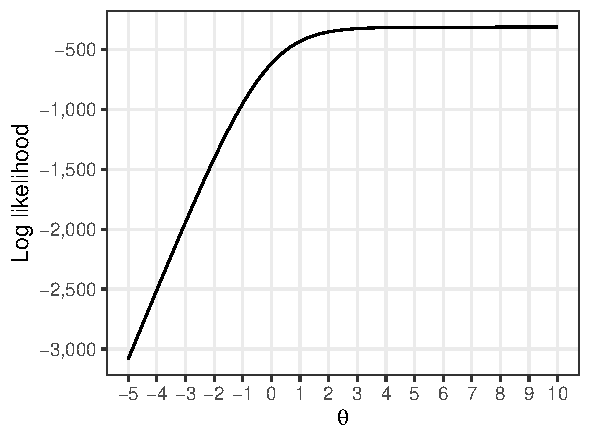
\includegraphics{graph/theta1} 

}

\caption{Likelihood of the scaled logit model as a function of \(\theta\) conditional on the \(\beta\) parameters set to their maximum likelihood estimates obtained from fitting the standard logistic model.}\label{fig:theta1}
\end{figure}

The reason why the likelihood flattens out is that the true baseline probability \(\lambda\) is \(1\) and any value of baseline log-odds \(\theta\) above around 5 corresponds to the baseline probability close to 1.

\pagebreak

\hypertarget{optimisation}{%
\section{Optimisation}\label{optimisation}}

Whatever algorithm is applied to the likelihood in Figure \ref{fig:theta1}, it will start walking toward larger and larger values of \(\theta\). The problem is that first (and second) derivatives of log-likelihood

\begin{align*}
\begin{bmatrix}
\frac{dl}{d\lambda} \\[6pt]
\frac{dl}{d\beta_j}
\end{bmatrix}
=
\begin{bmatrix}
\sum_i y_i - 
\frac{\text{exp}(\theta)}{1 + \text{exp}(\theta)} +
\frac{
(1 - y_i) \text{exp}(\boldsymbol{X_i}\boldsymbol{\beta}) \text{exp}(\theta)
}{
1 + \text{exp}(\boldsymbol{X_i}\boldsymbol{\beta}) 
\big( 1 + \text{exp}(\theta) \big)
}\\
\sum_i x_{j, i} \Big( -\frac{
\text{exp}(\boldsymbol{X_i}\boldsymbol{\beta}) 
}{
1 + \text{exp}(\boldsymbol{X_i}\boldsymbol{\beta})
} + \frac{
(1 - y_i) 
\text{exp}(\boldsymbol{X_i}\boldsymbol{\beta})
\big( 1 + \text{exp}(\theta) \big) 
}{
1 + \text{exp}(\boldsymbol{X_i}\boldsymbol{\beta}) 
\big( 1 + \text{exp}(\theta) \big)
} \Big) \\
\end{bmatrix}
\end{align*}

\begin{align*}
\begin{array}{cc}
\begin{matrix}
\frac{dl}{d\lambda} \qquad \qquad \qquad \qquad \qquad \qquad \qquad \qquad \qquad \qquad & \frac{dl}{d\beta_j}
\end{matrix}\\
\begin{matrix}
\frac{dl}{d\lambda} \\[6pt]
\frac{dl}{d\beta_j} \\
\end{matrix}
\begin{bmatrix}
\sum_i 
- \frac{
\text{exp}(\theta)
}{
\big( 1+\text{exp}(\theta) \big)^2
} +
\frac{
(1-y_i)(1+\text{exp}(\boldsymbol{X_i}\boldsymbol{\beta}))
\text{exp}(\boldsymbol{X_i}\boldsymbol{\beta}) \text{exp}(\theta)
}{
\Big( 1 + \text{exp}(\boldsymbol{X_i}\boldsymbol{\beta}) 
\big( 1 + \text{exp}(\theta) \big) \Big)^2
} &
\sum_i x_{j,i} \Big(
\frac{
(1-y_i)
\text{exp}(\boldsymbol{X_i}\boldsymbol{\beta}) \text{exp}(\theta)
}{
\Big( 1 + \text{exp}(\boldsymbol{X_i}\boldsymbol{\beta}) 
\big( 1 + \text{exp}(\theta) \big) \Big)^2
} \Big) \\
. &
\sum_i x_{j,i} \Big(
- \frac{
\text{exp}(\boldsymbol{X_i}\boldsymbol{\beta}) 
}{
\big( 1 + \text{exp}(\boldsymbol{X_i}\boldsymbol{\beta}) \big)^2
} + \frac{
(1-y_i)(1+\text{exp}(\theta))\text{exp}(\boldsymbol{X_i}\boldsymbol{\beta})
}{
\Big( 1 + \text{exp}(\boldsymbol{X_i}\boldsymbol{\beta}) 
\big( 1 + \text{exp}(\theta) \big) \Big)^2
} \Big) \\
\end{bmatrix}
\end{array}
\end{align*}

have \(e^\theta\) terms and at large values of \(\theta\) it becomes impossible to calculate some of them.

To overcome this problem I've implemented the gradient ascent algorithm (in addition to Newton-Raphson) which stops when the latest 20\% of iterations incremented the log-likelihood by less then \(0.001\).

Whenever Newton-Raphson fails to converge, gradient ascent will attempt to find the optimal set of estimates. This set can be used to calculate the maximum log-likelihood value of the scaled logit model and compare it to the maximum likelihood value of the standard logistic model fit to the same data. If the two values are (almost) the same then the addition of the baseline log-odds parameter \(\theta\) does not result in a better fit, therefore the baseline probability should be fixed to 1 by fitting (and inferring from) the standard logistic model.

I've implemented a function \texttt{check\_baseline} into the \texttt{sclr} package which fits the scaled logit and the logistic models and performs the likelihood ratio test to aid model selection.

\end{document}
